% Options for packages loaded elsewhere
\PassOptionsToPackage{unicode}{hyperref}
\PassOptionsToPackage{hyphens}{url}
\PassOptionsToPackage{dvipsnames,svgnames,x11names}{xcolor}
%
\documentclass[
  a4paperpaper,
  onecolumn]{article}

\usepackage{amsmath,amssymb}
\usepackage{iftex}
\ifPDFTeX
  \usepackage[T1]{fontenc}
  \usepackage[utf8]{inputenc}
  \usepackage{textcomp} % provide euro and other symbols
\else % if luatex or xetex
  \usepackage{unicode-math}
  \defaultfontfeatures{Scale=MatchLowercase}
  \defaultfontfeatures[\rmfamily]{Ligatures=TeX,Scale=1}
\fi
\usepackage{lmodern}
\ifPDFTeX\else  
    % xetex/luatex font selection
\fi
% Use upquote if available, for straight quotes in verbatim environments
\IfFileExists{upquote.sty}{\usepackage{upquote}}{}
\IfFileExists{microtype.sty}{% use microtype if available
  \usepackage[]{microtype}
  \UseMicrotypeSet[protrusion]{basicmath} % disable protrusion for tt fonts
}{}
\makeatletter
\@ifundefined{KOMAClassName}{% if non-KOMA class
  \IfFileExists{parskip.sty}{%
    \usepackage{parskip}
  }{% else
    \setlength{\parindent}{0pt}
    \setlength{\parskip}{6pt plus 2pt minus 1pt}}
}{% if KOMA class
  \KOMAoptions{parskip=half}}
\makeatother
\usepackage{xcolor}
\usepackage[left=2cm,top=2.5cm,right=2cm,bottom=2cm]{geometry}
\setlength{\emergencystretch}{3em} % prevent overfull lines
\setcounter{secnumdepth}{5}
% Make \paragraph and \subparagraph free-standing
\ifx\paragraph\undefined\else
  \let\oldparagraph\paragraph
  \renewcommand{\paragraph}[1]{\oldparagraph{#1}\mbox{}}
\fi
\ifx\subparagraph\undefined\else
  \let\oldsubparagraph\subparagraph
  \renewcommand{\subparagraph}[1]{\oldsubparagraph{#1}\mbox{}}
\fi


\providecommand{\tightlist}{%
  \setlength{\itemsep}{0pt}\setlength{\parskip}{0pt}}\usepackage{longtable,booktabs,array}
\usepackage{calc} % for calculating minipage widths
% Correct order of tables after \paragraph or \subparagraph
\usepackage{etoolbox}
\makeatletter
\patchcmd\longtable{\par}{\if@noskipsec\mbox{}\fi\par}{}{}
\makeatother
% Allow footnotes in longtable head/foot
\IfFileExists{footnotehyper.sty}{\usepackage{footnotehyper}}{\usepackage{footnote}}
\makesavenoteenv{longtable}
\usepackage{graphicx}
\makeatletter
\def\maxwidth{\ifdim\Gin@nat@width>\linewidth\linewidth\else\Gin@nat@width\fi}
\def\maxheight{\ifdim\Gin@nat@height>\textheight\textheight\else\Gin@nat@height\fi}
\makeatother
% Scale images if necessary, so that they will not overflow the page
% margins by default, and it is still possible to overwrite the defaults
% using explicit options in \includegraphics[width, height, ...]{}
\setkeys{Gin}{width=\maxwidth,height=\maxheight,keepaspectratio}
% Set default figure placement to htbp
\makeatletter
\def\fps@figure{htbp}
\makeatother

\usepackage{fancyhdr}
\pagestyle{fancy}
\fancyhead[R]{Erasmus+ Climatelabs}
\fancyhead[L]{
\includegraphics[width=2cm]{assets/logo-ENSGSI.png}}


\fancyfoot[L]{Document fait par: Fabio CRUZ}
\fancyfoot[C]{\thepage}
\fancyfoot[R]{ENSGSI - Version 25/10/2023}
\renewcommand{\footrulewidth}{1pt}% default is 0pt
\usepackage{mathtools}
\usepackage[makeroom]{cancel}
\usepackage{lscape}

\usepackage{booktabs}
\usepackage{longtable}
\usepackage{array}
\usepackage{multirow}
\usepackage{wrapfig}
\usepackage{float}
\usepackage{colortbl}
\usepackage{pdflscape}
\usepackage{tabu}
\usepackage{threeparttable}
\usepackage{threeparttablex}
\usepackage[normalem]{ulem}
\usepackage{makecell}
\usepackage{xcolor}
\makeatletter
\makeatother
\makeatletter
\makeatother
\makeatletter
\@ifpackageloaded{caption}{}{\usepackage{caption}}
\AtBeginDocument{%
\ifdefined\contentsname
  \renewcommand*\contentsname{Table of contents}
\else
  \newcommand\contentsname{Table of contents}
\fi
\ifdefined\listfigurename
  \renewcommand*\listfigurename{List of Figures}
\else
  \newcommand\listfigurename{List of Figures}
\fi
\ifdefined\listtablename
  \renewcommand*\listtablename{List of Tables}
\else
  \newcommand\listtablename{List of Tables}
\fi
\ifdefined\figurename
  \renewcommand*\figurename{Figure}
\else
  \newcommand\figurename{Figure}
\fi
\ifdefined\tablename
  \renewcommand*\tablename{Table}
\else
  \newcommand\tablename{Table}
\fi
}
\@ifpackageloaded{float}{}{\usepackage{float}}
\floatstyle{ruled}
\@ifundefined{c@chapter}{\newfloat{codelisting}{h}{lop}}{\newfloat{codelisting}{h}{lop}[chapter]}
\floatname{codelisting}{Listing}
\newcommand*\listoflistings{\listof{codelisting}{List of Listings}}
\makeatother
\makeatletter
\@ifpackageloaded{caption}{}{\usepackage{caption}}
\@ifpackageloaded{subcaption}{}{\usepackage{subcaption}}
\makeatother
\makeatletter
\@ifpackageloaded{tcolorbox}{}{\usepackage[skins,breakable]{tcolorbox}}
\makeatother
\makeatletter
\@ifundefined{shadecolor}{\definecolor{shadecolor}{rgb}{.97, .97, .97}}
\makeatother
\makeatletter
\makeatother
\makeatletter
\makeatother
\ifLuaTeX
  \usepackage{selnolig}  % disable illegal ligatures
\fi
\IfFileExists{bookmark.sty}{\usepackage{bookmark}}{\usepackage{hyperref}}
\IfFileExists{xurl.sty}{\usepackage{xurl}}{} % add URL line breaks if available
\urlstyle{same} % disable monospaced font for URLs
\hypersetup{
  pdftitle={Analyse de Sinchro},
  colorlinks=true,
  linkcolor={blue},
  filecolor={Maroon},
  citecolor={Blue},
  urlcolor={Blue},
  pdfcreator={LaTeX via pandoc}}

\title{Analyse de Sinchro}
\usepackage{etoolbox}
\makeatletter
\providecommand{\subtitle}[1]{% add subtitle to \maketitle
  \apptocmd{\@title}{\par {\large #1 \par}}{}{}
}
\makeatother
\subtitle{Projet Erasmus+ Climatelabs \textbar{} 2020 - 2023}
\author{}
\date{}

\begin{document}
\maketitle
\ifdefined\Shaded\renewenvironment{Shaded}{\begin{tcolorbox}[boxrule=0pt, borderline west={3pt}{0pt}{shadecolor}, frame hidden, sharp corners, interior hidden, breakable, enhanced]}{\end{tcolorbox}}\fi

\thispagestyle{fancy}

\textbf{Objectif:}

\begin{quote}
Cette document est une anlyse globale de l'outil Sinchro pour le Projet
Climatelabs piloté au sein de l'ENSGSI
\end{quote}

\hypertarget{temps-estimuxe9-selon-le-grant-agreement-du-projet}{%
\section{Temps estimé selon le Grant Agreement du
projet}\label{temps-estimuxe9-selon-le-grant-agreement-du-projet}}

\hypertarget{quantituxe9-de-jours-per-wp-initial}{%
\subsection{Quantité de jours per WP
initial}\label{quantituxe9-de-jours-per-wp-initial}}

\begin{table}[!h]
\centering\begingroup\fontsize{10}{12}\selectfont

\begin{tabular}[t]{llrr}
\toprule
WP & Role & Coût (Euros/Jour) & Jours (G.A.)\\
\midrule
 & Manager & 280 & 0\\

 & EC/Enseignant & 214 & 16\\

 & Technicien & 162 & 9\\

\multirow{-4}{*}{\raggedright\arraybackslash Preparation} & Administratif & 131 & 0\\
\cmidrule{1-4}
 & Manager & 280 & 6\\

 & EC/Enseignant & 214 & 47\\

 & Technicien & 162 & 35\\

\multirow{-4}{*}{\raggedright\arraybackslash Development} & Administratif & 131 & 0\\
\cmidrule{1-4}
 & Manager & 280 & 2\\

 & EC/Enseignant & 214 & 5\\

 & Technicien & 162 & 0\\

\multirow{-4}{*}{\raggedright\arraybackslash Quality Plan} & Administratif & 131 & 0\\
\cmidrule{1-4}
 & Manager & 280 & 1\\

 & EC/Enseignant & 214 & 19\\

 & Technicien & 162 & 2\\

\multirow{-4}{*}{\raggedright\arraybackslash Dissemination and Exploitation} & Administratif & 131 & 0\\
\cmidrule{1-4}
 & Manager & 280 & 2\\

 & EC/Enseignant & 214 & 8\\

 & Technicien & 162 & 10\\

\multirow{-4}{*}{\raggedright\arraybackslash Management} & Administratif & 131 & 10\\
\bottomrule
\end{tabular}
\endgroup{}
\end{table}

\hypertarget{quantituxe9-totale-de-jours-par-ruxf4le-dans-le-projet-selon-grant-agreement}{%
\subsection{Quantité totale de Jours par Rôle dans le projet selon Grant
Agreement}\label{quantituxe9-totale-de-jours-par-ruxf4le-dans-le-projet-selon-grant-agreement}}

\begin{table}[!h]
\centering\begingroup\fontsize{10}{12}\selectfont

\begin{tabular}[t]{lr}
\toprule
Role & Jours\\
\midrule
\cellcolor{gray!6}{Manager} & \cellcolor{gray!6}{11}\\
EC/Enseignant & 95\\
\cellcolor{gray!6}{Technicien} & \cellcolor{gray!6}{56}\\
Administratif & 10\\
\bottomrule
\end{tabular}
\endgroup{}
\end{table}

\hypertarget{ul-sinchro-janvier-2020---aouxfbt-2023}{%
\section{UL Sinchro: Janvier 2020 - Août
2023}\label{ul-sinchro-janvier-2020---aouxfbt-2023}}

Dans le tableau suivante, on identifie la quantité de jours par
participant et par tâche identifié sur Sinchro.

\begin{table}[H]
\centering
\resizebox{\linewidth}{!}{
\begin{tabular}[t]{lllrrrrrr|>{}r}
\toprule
WP & Task & Role & CLAUDINE & FABIO & FERNEY & LAURE & LAURENT & MAURICIO & Total\\
\midrule
 & WP 1.1 : Changemaker & EC & 3.0 & 18.25 &  & 4.0 & 1.50 & 4.50 & \textcolor{black}{\textbf{31.25}}\\
\cmidrule{2-10}
 & WP 1.1 : Changemaker & Tech &  & 1.75 & 6.00 &  &  &  & \textcolor{black}{\textbf{7.75}}\\
\cmidrule{2-10}
 & WP1.2 : Kick-­?Off & EC &  & 4.50 &  &  & 4.00 & 5.00 & \textcolor{black}{\textbf{13.50}}\\
\cmidrule{2-10}
 & WP1.2 : Kick-­?Off & Tech &  & 0.75 & 1.00 &  &  &  & \textcolor{black}{\textbf{1.75}}\\
\cmidrule{2-10}
 & WP1.3 : External & EC &  &  &  &  &  &  & \textcolor{black}{\textbf{}}\\
\cmidrule{2-10}
\multirow{-6}{*}{\raggedright\arraybackslash Preparation} & WP1.3 : External & Tech &  &  &  &  &  &  & \textcolor{black}{\textbf{}}\\
\cmidrule{1-10}
 & WP2.1: Social & EC &  &  &  &  &  &  & \textcolor{black}{\textbf{}}\\
\cmidrule{2-10}
 & WP2.1: Social & Man &  &  &  &  &  &  & \textcolor{black}{\textbf{}}\\
\cmidrule{2-10}
 & WP2.1: Social & Tech &  &  &  &  &  &  & \textcolor{black}{\textbf{}}\\
\cmidrule{2-10}
 & WP2.2 : Design and Development & EC & 7.0 & 18.75 &  & 2.0 &  & 15.25 & \textcolor{black}{\textbf{43.00}}\\
\cmidrule{2-10}
 & WP2.2 : Design and Development & Man &  & 4.00 &  &  &  &  & \textcolor{black}{\textbf{4.00}}\\
\cmidrule{2-10}
 & WP2.2 : Design and Development & Tech &  &  & 32.00 &  &  &  & \textcolor{black}{\textbf{32.00}}\\
\cmidrule{2-10}
 & WP2.4 : Applied Research Pilot & EC &  & 1.00 & 1.50 & 1.5 &  & 1.50 & \textcolor{black}{\textbf{5.50}}\\
\cmidrule{2-10}
 & WP2.4 : Applied Research Pilot & Man &  & 1.00 &  &  &  & 1.00 & \textcolor{black}{\textbf{2.00}}\\
\cmidrule{2-10}
\multirow{-9}{*}{\raggedright\arraybackslash Development} & WP2.4 : Applied Research Pilot & Tech &  &  & 4.00 &  &  &  & \textcolor{black}{\textbf{4.00}}\\
\cmidrule{1-10}
 & WP3 : Quality monitoring and E & EC &  & 4.00 & 1.00 &  &  &  & \textcolor{black}{\textbf{5.00}}\\
\cmidrule{2-10}
\multirow{-2}{*}{\raggedright\arraybackslash Quality Plan} & WP3 : Quality monitoring and E & Man &  & 1.50 &  &  &  & 1.00 & \textcolor{black}{\textbf{2.50}}\\
\cmidrule{1-10}
 & WP4.1 : Dissemination plan def & EC &  &  &  &  &  &  & \textcolor{black}{\textbf{}}\\
\cmidrule{2-10}
 & WP4.1 : Dissemination plan def & Man &  &  &  &  &  &  & \textcolor{black}{\textbf{}}\\
\cmidrule{2-10}
 & WP4.1 : Dissemination plan def & Tech &  &  &  &  &  &  & \textcolor{black}{\textbf{}}\\
\cmidrule{2-10}
 & WP4.2 : Latin American Applied & EC &  &  &  &  &  &  & \textcolor{black}{\textbf{}}\\
\cmidrule{2-10}
 & WP4.2 : Latin American Applied & Man &  &  &  &  &  &  & \textcolor{black}{\textbf{}}\\
\cmidrule{2-10}
 & WP4.2 : Latin American Applied & Tech &  &  &  &  &  &  & \textcolor{black}{\textbf{}}\\
\cmidrule{2-10}
 & WP4.3 : Outreach & EC & 2.5 & 5.25 &  & 6.5 &  & 3.00 & \textcolor{black}{\textbf{17.25}}\\
\cmidrule{2-10}
 & WP4.3 : Outreach & Man &  & 3.50 &  &  &  & 1.00 & \textcolor{black}{\textbf{4.50}}\\
\cmidrule{2-10}
 & WP4.3 : Outreach & Tech &  &  & 2.00 &  &  &  & \textcolor{black}{\textbf{2.00}}\\
\cmidrule{2-10}
 & WP4.4 : Design and Content Edi & EC &  & 1.50 &  &  & 2.25 &  & \textcolor{black}{\textbf{3.75}}\\
\cmidrule{2-10}
 & WP4.4 : Design and Content Edi & Man &  & 1.00 &  &  &  &  & \textcolor{black}{\textbf{1.00}}\\
\cmidrule{2-10}
\multirow{-12}{*}{\raggedright\arraybackslash Dissemination and Exploitation} & WP4.4 : Design and Content Edi & Tech &  &  & 1.00 &  &  &  & \textcolor{black}{\textbf{1.00}}\\
\cmidrule{1-10}
 & WP5 : Management and coordinat & EC & 2.0 & 6.00 &  & 0.5 & 0.50 & 1.00 & \textcolor{black}{\textbf{10.00}}\\
\cmidrule{2-10}
 & WP5 : Management and coordinat & Man &  & 3.00 &  &  &  &  & \textcolor{black}{\textbf{3.00}}\\
\cmidrule{2-10}
 & WP5 : Management and coordinat & Tech &  & 1.00 & 13.25 &  &  &  & \textcolor{black}{\textbf{14.25}}\\
\cmidrule{2-10}
\multirow{-4}{*}{\raggedright\arraybackslash Management} & WP5 : Management and coordinat & Admin &  & 0.50 & 11.00 &  &  &  & \textcolor{black}{\textbf{11.50}}\\
\bottomrule
\end{tabular}}
\end{table}

\hypertarget{jours-duxe9clares-en-sinchro-pour-le-projet-climatelabs}{%
\subsection{Jours déclares en Sinchro pour le projet
ClimateLabs}\label{jours-duxe9clares-en-sinchro-pour-le-projet-climatelabs}}

\begin{table}[H]
\centering\begingroup\fontsize{10}{12}\selectfont

\begin{tabular}[t]{llr}
\toprule
WP & Role & Sincro.UL\\
\midrule
\cellcolor{gray!6}{Preparation} & \cellcolor{gray!6}{EC} & \cellcolor{gray!6}{44.75}\\
\cmidrule{1-3}
Preparation & Tech & 9.50\\
\cmidrule{1-3}
\cellcolor{gray!6}{Development} & \cellcolor{gray!6}{Man} & \cellcolor{gray!6}{6.00}\\
\cmidrule{1-3}
Development & EC & 48.50\\
\cmidrule{1-3}
\cellcolor{gray!6}{Development} & \cellcolor{gray!6}{Tech} & \cellcolor{gray!6}{36.00}\\
\cmidrule{1-3}
Quality Plan & Man & 2.50\\
\cmidrule{1-3}
\cellcolor{gray!6}{Quality Plan} & \cellcolor{gray!6}{EC} & \cellcolor{gray!6}{5.00}\\
\cmidrule{1-3}
Dissemination and Exploitation & Man & 5.50\\
\cmidrule{1-3}
\cellcolor{gray!6}{Dissemination and Exploitation} & \cellcolor{gray!6}{EC} & \cellcolor{gray!6}{21.00}\\
\cmidrule{1-3}
Dissemination and Exploitation & Tech & 3.00\\
\cmidrule{1-3}
\cellcolor{gray!6}{Management} & \cellcolor{gray!6}{Man} & \cellcolor{gray!6}{3.00}\\
\cmidrule{1-3}
Management & EC & 10.00\\
\cmidrule{1-3}
\cellcolor{gray!6}{Management} & \cellcolor{gray!6}{Tech} & \cellcolor{gray!6}{14.25}\\
\cmidrule{1-3}
Management & Admin & 11.50\\
\bottomrule
\end{tabular}
\endgroup{}
\end{table}

\hypertarget{differences-entre-jours-de-ga-et-jours-declaruxe9s-sur-sinchro}{%
\subsection{Differences entre Jours de GA et Jours declarés sur
Sinchro}\label{differences-entre-jours-de-ga-et-jours-declaruxe9s-sur-sinchro}}

\begin{table}[H]
\centering
\begin{tabular}[t]{llrr|>{}r}
\toprule
WP & Role & Jours.GA & Sincro.UL & Difference\\
\midrule
\cellcolor{gray!6}{Preparation} & \cellcolor{gray!6}{Man} & \cellcolor{gray!6}{0} & \cellcolor{gray!6}{} & \textcolor{black}{\textbf{\cellcolor{gray!6}{}}}\\
\cmidrule{1-5}
Preparation & EC & 16 & 44.75 & \textcolor{black}{\textbf{28.75}}\\
\cmidrule{1-5}
\cellcolor{gray!6}{Preparation} & \cellcolor{gray!6}{Tech} & \cellcolor{gray!6}{9} & \cellcolor{gray!6}{9.50} & \textcolor{black}{\textbf{\cellcolor{gray!6}{0.50}}}\\
\cmidrule{1-5}
Preparation & Admin & 0 &  & \textcolor{black}{\textbf{}}\\
\cmidrule{1-5}
\cellcolor{gray!6}{Development} & \cellcolor{gray!6}{Man} & \cellcolor{gray!6}{6} & \cellcolor{gray!6}{6.00} & \textcolor{black}{\textbf{\cellcolor{gray!6}{0.00}}}\\
\cmidrule{1-5}
Development & EC & 47 & 48.50 & \textcolor{black}{\textbf{1.50}}\\
\cmidrule{1-5}
\cellcolor{gray!6}{Development} & \cellcolor{gray!6}{Tech} & \cellcolor{gray!6}{35} & \cellcolor{gray!6}{36.00} & \textcolor{black}{\textbf{\cellcolor{gray!6}{1.00}}}\\
\cmidrule{1-5}
Development & Admin & 0 &  & \textcolor{black}{\textbf{}}\\
\cmidrule{1-5}
\cellcolor{gray!6}{Quality Plan} & \cellcolor{gray!6}{Man} & \cellcolor{gray!6}{2} & \cellcolor{gray!6}{2.50} & \textcolor{black}{\textbf{\cellcolor{gray!6}{0.50}}}\\
\cmidrule{1-5}
Quality Plan & EC & 5 & 5.00 & \textcolor{black}{\textbf{0.00}}\\
\cmidrule{1-5}
\cellcolor{gray!6}{Quality Plan} & \cellcolor{gray!6}{Tech} & \cellcolor{gray!6}{0} & \cellcolor{gray!6}{} & \textcolor{black}{\textbf{\cellcolor{gray!6}{}}}\\
\cmidrule{1-5}
Quality Plan & Admin & 0 &  & \textcolor{black}{\textbf{}}\\
\cmidrule{1-5}
\cellcolor{gray!6}{Dissemination and Exploitation} & \cellcolor{gray!6}{Man} & \cellcolor{gray!6}{1} & \cellcolor{gray!6}{5.50} & \textcolor{black}{\textbf{\cellcolor{gray!6}{4.50}}}\\
\cmidrule{1-5}
Dissemination and Exploitation & EC & 19 & 21.00 & \textcolor{black}{\textbf{2.00}}\\
\cmidrule{1-5}
\cellcolor{gray!6}{Dissemination and Exploitation} & \cellcolor{gray!6}{Tech} & \cellcolor{gray!6}{2} & \cellcolor{gray!6}{3.00} & \textcolor{black}{\textbf{\cellcolor{gray!6}{1.00}}}\\
\cmidrule{1-5}
Dissemination and Exploitation & Admin & 0 &  & \textcolor{black}{\textbf{}}\\
\cmidrule{1-5}
\cellcolor{gray!6}{Management} & \cellcolor{gray!6}{Man} & \cellcolor{gray!6}{2} & \cellcolor{gray!6}{3.00} & \textcolor{black}{\textbf{\cellcolor{gray!6}{1.00}}}\\
\cmidrule{1-5}
Management & EC & 8 & 10.00 & \textcolor{black}{\textbf{2.00}}\\
\cmidrule{1-5}
\cellcolor{gray!6}{Management} & \cellcolor{gray!6}{Tech} & \cellcolor{gray!6}{10} & \cellcolor{gray!6}{14.25} & \textcolor{black}{\textbf{\cellcolor{gray!6}{4.25}}}\\
\cmidrule{1-5}
Management & Admin & 10 & 11.50 & \textcolor{black}{\textbf{1.50}}\\
\bottomrule
\end{tabular}
\end{table}

\hypertarget{differences-totale-entre-jours-du-ga-et-jours-declaruxe9s-sur-sinchro-par-ruxf4le}{%
\subsection{Differences totale entre Jours du GA et Jours declarés sur
Sinchro par
Rôle}\label{differences-totale-entre-jours-du-ga-et-jours-declaruxe9s-sur-sinchro-par-ruxf4le}}

Le tableau montre les jours additionels que l'UL a travaillé dans le
projet comme co-financement avec des ressources propres.

\begin{table}[H]
\centering\begingroup\fontsize{10}{12}\selectfont

\begin{tabular}[t]{lrr|>{}r}
\toprule
Role & Jours GA & Jours UL Sinchro & Difference\\
\midrule
\cellcolor{gray!6}{Man} & \cellcolor{gray!6}{11} & \cellcolor{gray!6}{17.00} & \textcolor{black}{\textbf{\cellcolor{gray!6}{6.00}}}\\
EC & 95 & 129.25 & \textcolor{black}{\textbf{34.25}}\\
\cellcolor{gray!6}{Tech} & \cellcolor{gray!6}{56} & \cellcolor{gray!6}{62.75} & \textcolor{black}{\textbf{\cellcolor{gray!6}{6.75}}}\\
Admin & 10 & 11.50 & \textcolor{black}{\textbf{1.50}}\\
\bottomrule
\end{tabular}
\endgroup{}
\end{table}

\hypertarget{graphique-des-distribution-des-jours-dans-le-projet}{%
\subsection{Graphique des distribution des jours dans le
projet}\label{graphique-des-distribution-des-jours-dans-le-projet}}

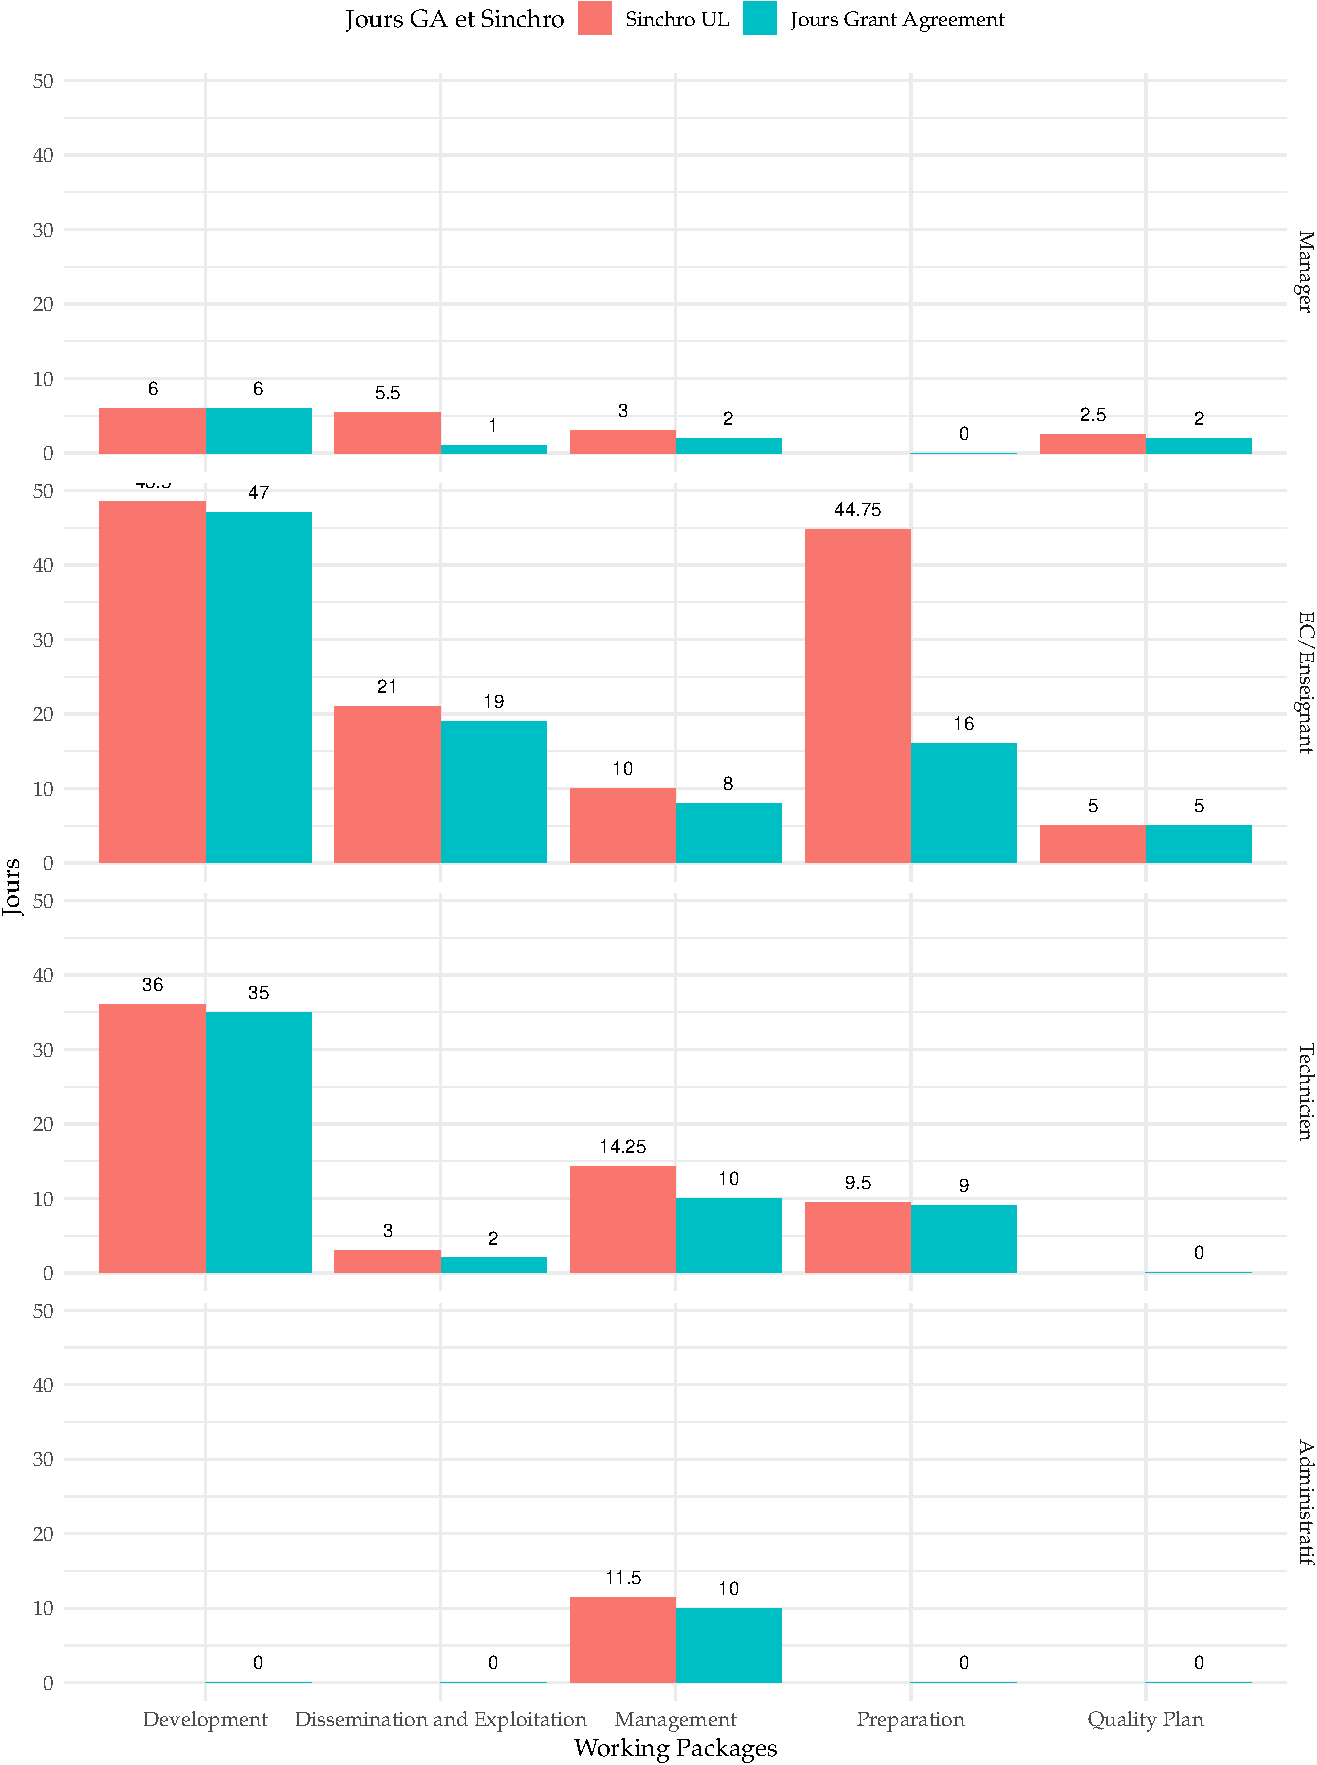
\includegraphics[width=0.9\textwidth,height=\textheight]{admin_files/figure-pdf/unnamed-chunk-8-1.pdf}



\end{document}
